\section[SDL]{La bibliothèque SDL}

\subsection{Fonctionnement de SDL} %%%%%%%%%%%%%%%%%%%%%%%%%%%%%%%%%%%%%%%%%%%%
\begin{frame}
	\begin{center}
		\huge
		La bibliothèque SDL
	\end{center}
\end{frame}

\begin{frame}
	\frametitle{Le principe actif SDL}
	\begin{center}
		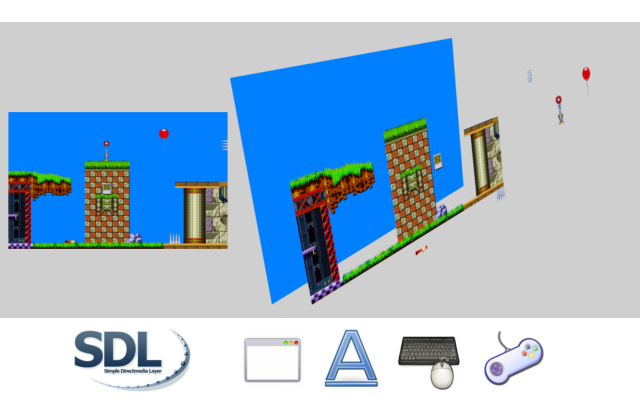
\includegraphics[width=9cm]{pics/sdlSurfaces.png}
	\end{center}
\end{frame}

\begin{frame}[fragile]
	\frametitle{Les modules SDL}
	\begin{center}
		\begin{minipage}{0.4\textwidth}
			\begin{itemize}
				\item ~~~sdl
			\end{itemize}
		\end{minipage}
	\end{center}
	\begin{center}
		\begin{minipage}{0.4\textwidth}
			\begin{itemize}
				\item Sdlwm
				\item Sdlvideo
				\item Sdltime
				\item Sdlevent
			\end{itemize}
		\end{minipage}
		\begin{minipage}{0.4\textwidth}
			\begin{itemize}
				\item Sdlttf
				\item Sdlloader
				\item Sdlmixer
				\item Sdlgfx
			\end{itemize}
		\end{minipage}
	\end{center}
\end{frame}

\subsection{Introduction à SDL} %%%%%%%%%%%%%%%%%%%%%%%%%%%%%%%%%%%%%%%%%%%%%%%

\begin{frame}[fragile]
	\frametitle{Initialisation de SDL}
	\begin{minipage}{0.55\textwidth}
		\textbf{L'intialisation de base}
		\lstset{basicstyle=\small}
		\begin{lstlisting}
  Sdl.init [`EVERYTHING] 
		\end{lstlisting}
		\textbf{L'intialisation et ouverture d'une fenetre}
		\lstset{basicstyle=\small}
		\begin{lstlisting}
  Sdl.init [`EVERYTHING]

  let screen = 
   Sdlvideo.set_video_mode 
   ~w ~h ~bpp [`HWSURFACE]
		\end{lstlisting}
	\end{minipage}
	\begin{minipage}{0.4\textwidth}
		\begin{itemize}
			\item `AUDIO
			\item `CDROM
			\item `JOYSTICK
			\item `TIMER
			\item `VIDEO
		\end{itemize}
		\begin{itemize}
			\item `EVERYTHING
		\end{itemize}
	\end{minipage}
\end{frame}

\subsection{L'affichage bas niveau} %%%%%%%%%%%%%%%%%%%%%%%%%%%%%%%%%%%%%%%%%%%

\begin{frame}[fragile]
	\frametitle{Quelques mots sur les surfaces}
	\begin{minipage}{0.55\textwidth}
		\lstset{basicstyle=\small}
		\begin{lstlisting}
type surface_info = {
  flags : surface_flags list;
  w : int;
  h : int;
  pitch : int;
  clip_rect : rect;
  refcount : int;
}
		\end{lstlisting}
	\end{minipage}
	\begin{minipage}{0.4\textwidth}
		\begin{itemize}
			\item `DOUBLEBUF
			\item `FULLSCREEN
			\item `HWSURFACE
			\item `OPENGL
			\item `SWSURFACE
			\item `SRCALPHA
		\end{itemize}
	\end{minipage}
\end{frame}


\begin{frame}
	\frametitle{La surface de type \textit{Double Buffer}}
	\begin{center}
		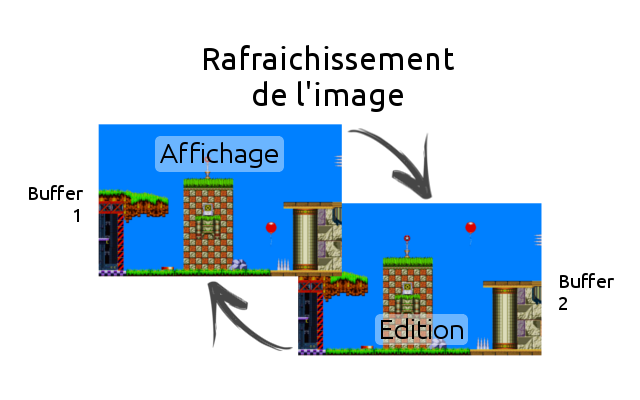
\includegraphics[width=9cm]{pics/doubleBuffer.png}
	\end{center}
\end{frame}

\begin{frame}[fragile]
	\frametitle{Le type rect}
	\begin{center}\begin{minipage}{0.4\textwidth}
		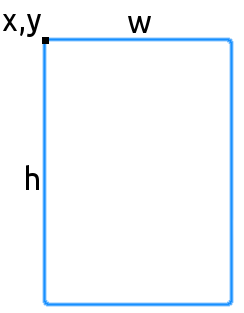
\includegraphics[width=3cm]{pics/rect.png}
	\end{minipage}
	\begin{minipage}{0.4\textwidth}
		\lstset{basicstyle=\footnotesize}
		\begin{lstlisting}
type rect = {
  mutable r_x : int;
  mutable r_y : int;
  mutable r_w : int;
  mutable r_h : int;
} 
		\end{lstlisting}
	\end{minipage}\end{center}
	\lstset{basicstyle=\footnotesize}
	\begin{lstlisting}
val rect : x:int -> y:int -> w:int -> h:int -> rect

val surface_dims : surface -> int * int * int
	\end{lstlisting}
\end{frame}

\begin{frame}[fragile]
	\frametitle{Le chargement d'image}
	\textbf{Charger/Sauver une image .bmp}
	\begin{lstlisting}
  val load_BMP : string -> surface
  val save_BMP : surface -> string -> unit
	\end{lstlisting}
	\textbf{Charger une image .\{jpeg,png,tiff\}}
	\begin{lstlisting}
  val Sdlloader.load_image : 
    string -> surface

	\end{lstlisting}
\end{frame}

\begin{frame}
	\frametitle{Les pixels...}
	\begin{center}
		
\includegraphics[width=9cm]{pics/Joconde-pixel.jpg}
	\end{center}
\end{frame}

\begin{frame}[fragile]
	\frametitle{La couleur}
	\begin{lstlisting}
type color = int * int * int
let c = ((255,255,255):color)

val map_RGB : 
  surface -> ?alpha:int -> color -> int32
val get_RGB : surface -> int32 -> color
val get_RGBA : 
  surface -> int32 -> color * int
	\end{lstlisting}
\end{frame}

\begin{frame}[fragile]
	\frametitle{La transparance \textbf{globale} des surfaces}
	\textit{Modifie la transparance de tout les pixel de la surface}
	\begin{lstlisting}
val set_color_key : 
  surface -> ?rle:bool -> int32 -> unit
val get_color_key : surface -> int32
val unset_color_key

val unset_alpha : surface -> unit
val set_alpha : 
  surface -> ?rle:bool -> int -> unit
val get_alpha : surface -> int
	\end{lstlisting}
\end{frame}

\begin{frame}[fragile]
	\frametitle{\og{}Bon ! Quand est-ce qu'on manipule des pixels ?\fg}
	\begin{lstlisting}
val lock : surface -> unit
val unlock : surface -> unit
val must_lock : surface -> bool

val get_pixel : 
  surface -> x:int -> y:int -> int32
val get_pixel_color : 
  surface -> x:int -> y:int -> color

val put_pixel : 
  surface -> x:int -> y:int -> int32 -> unit
val put_pixel_color : 
  surface -> x:int -> y:int -> color -> unit
	\end{lstlisting}
\end{frame}

\begin{frame}[fragile]
	\frametitle{\og{}Merge Down !\fg}
	\begin{center}
		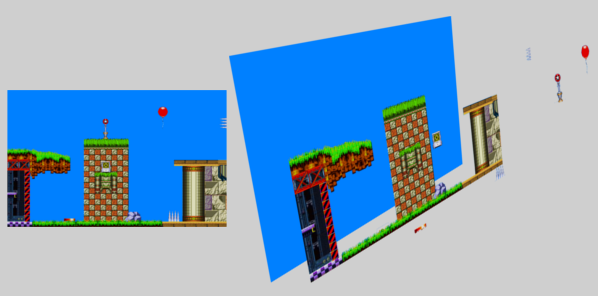
\includegraphics[width=3.6cm]{pics/surfacesMerge.png}
	\end{center}
	\begin{lstlisting}
val fill_rect : 
  ?rect:rect -> surface -> int32 -> unit

val blit_surface : 
  src:surface -> ?src_rect:rect -> 
  dst:surface -> ?dst_rect:rect -> 
  unit -> unit

val display_format : 
  ?alpha:bool -> surface -> surface
	\end{lstlisting}
\end{frame}

\begin{frame}[fragile]
	\frametitle{L'actualisation de l'affichage}

\end{frame}
